\begin{figure}[h]
    \centering
    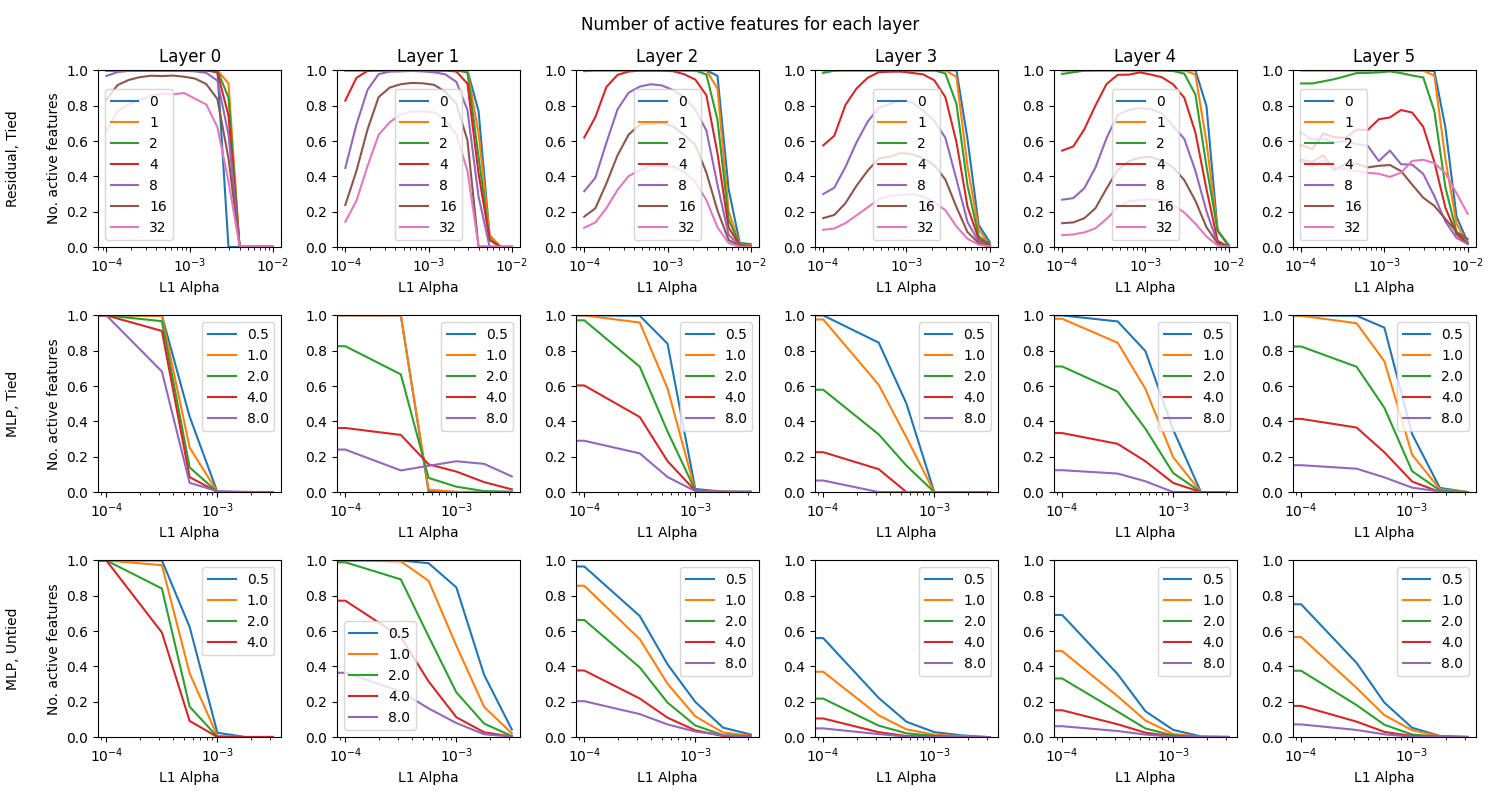
\includegraphics[width=0.9\textwidth]{images/n_active_summary.png}
    \caption{The number of features that are active, defined as activating more than 10 times across 10M datapoints, changes with sparsity hyperparamter $\alpha$ and dictionary size ratio $R$.}
    \label{fig:n_active_summary}
\end{figure}

In Figure \ref{fig:n_active_summary} we see that, for residual streams, we consistently learn dictionaries that are at least 4x overcomplete before some features start to drop out completely, with the correct hyperparameters. For MLP layers you see large numbers of dead features even with hyperparameter $\alpha=0$. These figures informed the selection of $\alpha=8.6e-4$ and $\alpha=3.2e-4$ that went into the graphs in Section \ref{section:autointerp} for the residual stream and MLP respectively. Due to the large part of the input space that is never used due to the non-linearity, it is much easier for MLP dictionary features to become stuck at a position where they hardly ever activate. In future we plan to reinitialise such `dead features' to ensure that we learn as many useful dictionary features as possible.